\documentclass{amsart}
\usepackage[utf8]{inputenc}
\usepackage{graphicx}

\title{Fritter Design \\ For a more potato-ey tomorrow}
\author{Evan Lynch}
\date{October 1, 2014}

\begin{document}
\maketitle
\section{Terminology}
Since this is \emph{Fritter} and not \emph{Twitter}, the \emph{Tweet} analog is
called a  \emph{Frite}. To deliver a \emph{Frite},
one must \emph{Fry} it, making the deliverer a \emph{Fryer}. Additionally, since one often
pays for a potato with dollars and cents, to tag a \emph{Frite} one would use a 
``\$cashtag.'' If one found a \emph{Frite} to their liking and wanted to \emph{Fry} it
themselves without modification, this would be called \emph{refry}-ing.

\section{Highlights}
\label{sec:subtitle}
The potato spinner GIF that shows up when the UI is blocking is the clear winner. However, another
highlight is the simple API. The API is good because it is fully specified in terms of inputs, outputs, and side-effects, and though limited in scope, it is designed without a particular client in mind. This made
writing the REACT client-side app much easier.

\section{Design Challenges}
\label{sec:another_subtitle}
The main design decisions to make were the following.
\begin{enumerate}
\item What schema to select for the data model
\item How much view rendering to do client-side / what view end-points to support
\item What interface to expose through an API to the client
\item How to model data on the client side
\item How to render views on the client side
\end{enumerate}
Now, I will describe the decision I made for each and why.

\subsection{Data Model}
I chose to use the mongoose wrapper for MongoDB. The data model consists of two schema
defined in model.js.
\begin{verbatim}
User:
    username: String
    hash: String
    apiID: String of the form u_??????????

Frite:
    text: String
    timestamp: Date (serialized by mongoose)
    apiID: String of the form fr_??????????
    cashtags: Array of Strings
    user: Number (ObjectID referencing users collection) --- ``poster''
    refry: Number (ObjectID referencing users collection) --- ``author''
\end{verbatim}
Much of these schema are obvious; however, two decisions stand out. First, each Frite
carries a reference to a User document rather than a nested user to allow users to
change their usernames, passwords, etc. in the future.

Second, when a Frite is refried (``retweeted''), a new Frite is created with the
original Frite's text and the refry field set to the original Frite's user. Another option
would have been to store a separate kind of object instead of a full Frite which would
references the original Frite. The choice to save only the original Frite's user
was made to simplify the data model (no recursive structure) and to avoid confusing
situatiosn like when the original Frite is edited (should the refrys change to?), etc.

However, Frites are mutable and we don't want to allow a user to refry a Frite and then
change the text (essentially attributing their own words to someone else). Therefore,
we have to maintain the invariant that the
refry field of a Frite is only set to a user if the text of the Frite corresponds to the text
of another Frite which that user at one point made. This is a hard invariant to verify, but
easy to maintain and was kept in mind when implementing the API.

Finally, the data model was selected so that only one mongoose.populate call would
need to be made to get a complete picture of a Frite.

\subsection{Views}
I opted to do the vast majority of view rendering on the client side. The server only
responds with HTML at two end-points ``/'' and ``/login'' routed in views.js.
The ``/login'' end-point
allows a user to log in regardless of what username is set in the session while the
``/'' end-point goes to the main site unless there is no username set in the session
in which case it goes to the login page. The HTML response on both of these do little
more than load the client-side javascript and set globally scoped variable ``bootstrap''
in which it passes the username from the session. For the small amount of templating
this required, I used the Jade template engine.


\subsection{API}
The API was designed as a ``public'' API taking the perspective that any API that the
server presents as an interface is ``public'' to begin with in the sense that anyone
can send it requests not just the designated client app. Therefore, it sends and
receives JSON and attempts to return helpful error messages and status codes when
requests are formatted wrong or fail for other reasons. The interface is well documented
in api.js.


\subsection{Client-side}
I chose to use Backbone.js for storing a model of responses from the API in the client app. I use
little of Backbone's functionality otherwise, but the Backbone model was a convenient choice for
parsing performing API fetches and saving them in a coherent manner and keeping them in sorted order.

The client implements the view with REACT.js which is a framework for writing reactive client-side
applications in a declarative fashion. The structure of a view in REACT is a hierarchy of components
each which can carry and update state as well as pass down properties to children. The UI is declared
to appear a certain way based on the state and properties that the component has. My REACT code has
the following structure.
\begin{figure}[htbp]
    \centering
    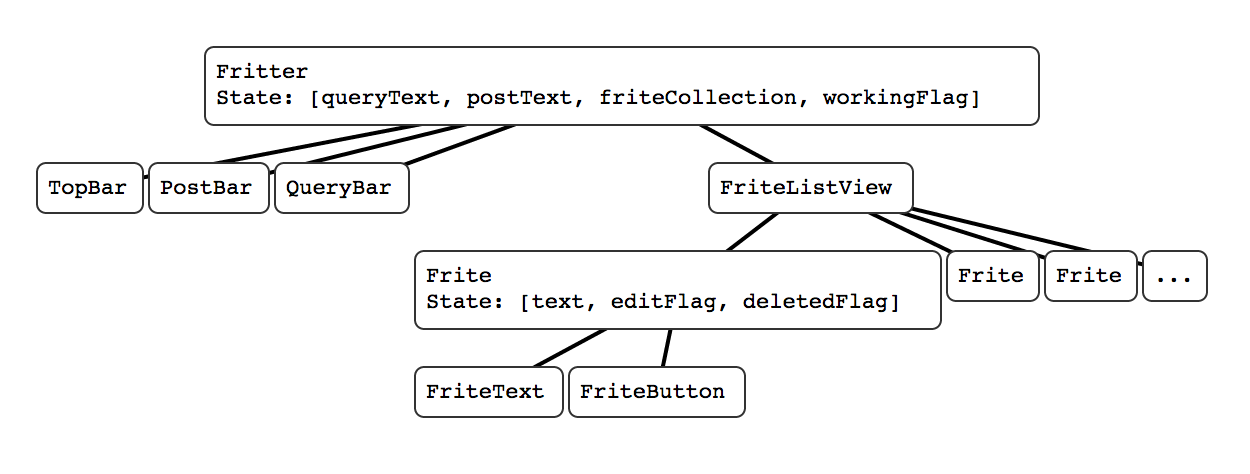
\includegraphics[width=0.95\textwidth]{reacttree}
\end{figure}


\end{document}